\documentclass{beamer}[10]

\usepackage{graphicx}
\usepackage{xcolor}
\usepackage{tabto}
%\usepackage{beamerthemesplit}
\usepackage{tikz}
\usepackage{cancel}
\usepackage{verbatim}
\usepackage{fancybox}
\usepackage{enumerate}
\usepackage{amsmath,amssymb,amsthm,textcomp,mathtools}
\usepackage[super]{nth}
\usepackage[amssymb]{SIunits}
\usepackage{booktabs}
\usepackage{cancel}
\usepackage{bm}
\usepackage[utf8]{inputenc}
\usepackage{tabularx}
\usepackage{ragged2e}
\newcolumntype{Y}{ >{\RaggedRight\arraybackslash}X}
\usetikzlibrary{arrows,shapes}
\newcommand\T{\rule{0pt}{2.6ex}}
\newcommand\B{\rule[-1.2ex]{0pt}{0pt}}
\definecolor{UUcrimson}{RGB}{204,0,0}
\mode<presentation>
{ \usetheme{default}
  \usecolortheme[named=UUcrimson]{structure}
  \useinnertheme{circles}
  \setbeamercovered{transparent}
  \setbeamertemplate{blocks}[rounded]
  \usefonttheme[onlymath]{serif}
  \setbeamertemplate{navigation symbols}{}
  \setbeamertemplate{footline}[page number]
  \setbeamertemplate{navigation symbols}{}
  \setbeamercolor{section in toc}{fg=black,bg=white}
  \setbeamercolor{alerted text}{fg=UUcrimson!80!gray}
  \setbeamercolor*{palette primary}{fg=white,bg=UUcrimson}
  \setbeamercolor*{palette secondary}{fg=UUcrimson!70!black,bg=gray!15!white}
  \setbeamercolor*{palette tertiary}{bg=UUcrimson!80!black,fg=gray!10!white}
  \setbeamercolor*{palette quaternary}{fg=UUcrimson,bg=gray!5!white}
  \setbeamercolor*{palette sidebar primary}{fg=UUcrimson!10!black}
  \setbeamercolor*{palette sidebar secondary}{fg=white}
  \setbeamercolor*{palette sidebar tertiary}{fg=UUcrimson!50!black}
  \setbeamercolor*{palette sidebar quaternary}{fg=gray!10!white}
  \setbeamercolor{titlelike}{parent=palette primary,fg=white}
  \setbeamercolor{frametitle}{bg=UUcrimson}
  \setbeamercolor{frametitle right}{bg=UUcrimson}
  \setbeamercolor*{separation line}{}
  \setbeamercolor*{fine separation line}{}
}

\usetikzlibrary{backgrounds}
\makeatletter
\tikzstyle{every picture}+=[remember picture]
\tikzset{%
  fancy quotes/.style={
    text width=\fq@width pt,
    align=justify,
    inner sep=1em,
    anchor=north west,
    minimum width=\linewidth,
    font=\itshape
  },
  fancy quotes width/.initial={.8\linewidth},
  fancy quotes marks/.style={
    scale=8,
    text=white,
    inner sep=0pt,
  },
  fancy quotes opening/.style={
    fancy quotes marks,
  },
  fancy quotes closing/.style={
    fancy quotes marks,
  },
  fancy quotes background/.style={
    show background rectangle,
    inner frame xsep=0pt,
    background rectangle/.style={
      fill=gray!25,
      rounded corners,
    },
  }
}
\newenvironment{fancyquotes}[1][]{%
\noindent
\tikzpicture[fancy quotes background]
\node[fancy quotes opening,anchor=north west] (fq@ul) at (0,0) {``};
\tikz@scan@one@point\pgfutil@firstofone(fq@ul.east)
\pgfmathsetmacro{\fq@width}{\linewidth - 2*\pgf@x}
\node[fancy quotes,#1] (fq@txt) at (fq@ul.north west) \bgroup}
{\egroup;
\node[overlay,fancy quotes closing,anchor=east] at (fq@txt.south east) {''};
\endtikzpicture}
\makeatother

\usepackage{scalerel}[2014/03/10]
\usepackage{stackengine}
\usepackage{empheq}
\newcommand*\widefbox[1]{\fbox{\hspace{0.5em}#1\hspace{0.5em}}}

\newcommand\reallywidetilde[1]{\ThisStyle{%
  \setbox0=\hbox{$\SavedStyle#1$}%
  \stackengine{-.1\LMpt}{$\SavedStyle#1$}{%
    \stretchto{\scaleto{\SavedStyle\mkern.2mu\sim}{.5467\wd0}}{.4\ht0}%
%    .2mu is the kern imbalance when clipping white space
%    .5467++++ is \ht/[kerned \wd] aspect ratio for \sim glyph
  }{O}{c}{F}{T}{S}%
}}
\usepackage{media9}

\logo{
\includegraphics[width=0.75cm]{logo.jpg}}
\author[Gibbs]{Dr. Jeremy A. Gibbs}
\institute{Department of Mechanical Engineering\\University of Utah}
\date{Fall 2016}
\title{LES of Turbulent Flows: Lecture 10}

\begin{document}

%----------------------------------------------------------------------------------------
%	TITLE & TOC SLIDES
%----------------------------------------------------------------------------------------

\begin{frame} 
  \titlepage
\end{frame}

%------------------------------------------------

\begin{frame}
\frametitle{Overview}
\tableofcontents
\end{frame}

%------------------------------------------------
\section{Turbulence modeling (alternative strategies) } %
%------------------------------------------------

\begin{frame}{Turbulence modeling (alternative strategies)}

\begin{itemize}
	\item Our discussion of turbulence modeling has centered around separating the flow into resolved and SFSs
	\item We have focused on using a low-pass filtering operation to accomplish this separation
	\item The goal of this procedure is to reduce the number of degrees of freedom in our numerical solution -- \textit{i.e.}, make them more computationally affordable
	\item This is not the only way to accomplish complexity reduction in a turbulent flow
	\item We will briefly review a couple of different methods
\end{itemize}

\end{frame}

%------------------------------------------------
\subsection{Coherent Vortex Simulations (CVS)}
%------------------------------------------------

\begin{frame}{Coherent Vortex Simulations (CVS)}

\begin{itemize}
	\item See Farge and Schneider (2001) on Canvas or class website
	\item The idea of CVS is that the turbulent flow field is decomposed into coherent (organized) and incoherent (random) components.
	\item The decomposition is accomplished by using either a continuous or orthonormal wavelet filter
\end{itemize}

\end{frame}

%------------------------------------------------

\begin{frame}{Coherent Vortex Simulations (CVS)}

\begin{itemize}
	\item CVS, like LES, is classified as a semi-deterministic turbulence simulation method
	\item It is called semi-deterministic because some degrees of freedom are explicitly (deterministically) computed while the influence of others is modeled.
	\item DNS is considered fully deterministic since all scales of motion are resolved
	\item RANS is a fully statistical approach since only the steady solution of the mean flow field is solved deterministically, while the impact of all fluctuations are modeled
\end{itemize}

\end{frame}

%------------------------------------------------

\begin{frame}{Coherent Vortex Simulations (CVS)}
\begin{figure}
	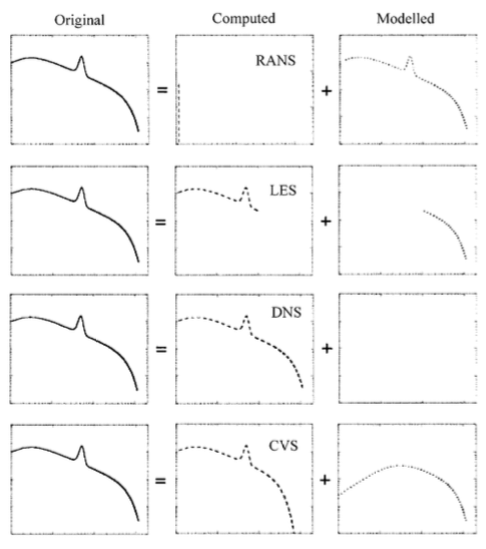
\includegraphics[width=0.6\textwidth]{cvs1}
	\caption{Methods to compute turbulent flows. Adapted from Farge and Schneider (2001).}
\end{figure}
\end{frame}

%------------------------------------------------

\begin{frame}{Coherent Vortex Simulations (CVS)}

\begin{itemize}
	\item For CVS, a nonlinear wavelet filter is applied to the N-S equations
	\item Coherent vortices are extracted without the need to impose an \textit{a priori} cut-off scale -- unlike, \textit{e.g.}, LES
	\item The only \textit{a priori} requirement is that the random (filtered-out) motions have a $\sim$Gaussian PDF
\end{itemize}
\end{frame}

%------------------------------------------------

\begin{frame}{Coherent Vortex Simulations (CVS)}

\begin{itemize}
	\item In principle, the CVS approach deterministically solves the evolution of coherent vortices in a wavelet basis (we will review this in a minute)
	\item The wavelet basis adapts to regions of strong gradients
	\item Thus, CVS resolves the nonlinear interactions of coherent vortices
	\item Nonlinear vortex interactions lead to incoherent motions -- these motions must be modeled 
\end{itemize}

\end{frame}

%------------------------------------------------

\begin{frame}{Coherent Vortex Simulations (CVS)}
\begin{figure}
	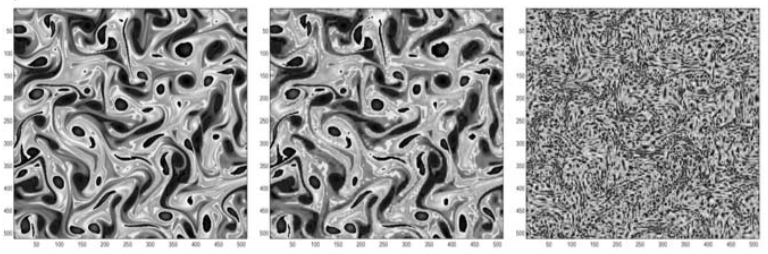
\includegraphics[width=1\textwidth]{cvs2}
	\caption{Total (left), coherent (center), and incoherent vorticity (right). From Farge and Schneider (2001).}
\end{figure}
\end{frame}

%------------------------------------------------

\begin{frame}{Coherent Vortex Simulations (CVS)}
\begin{figure}
	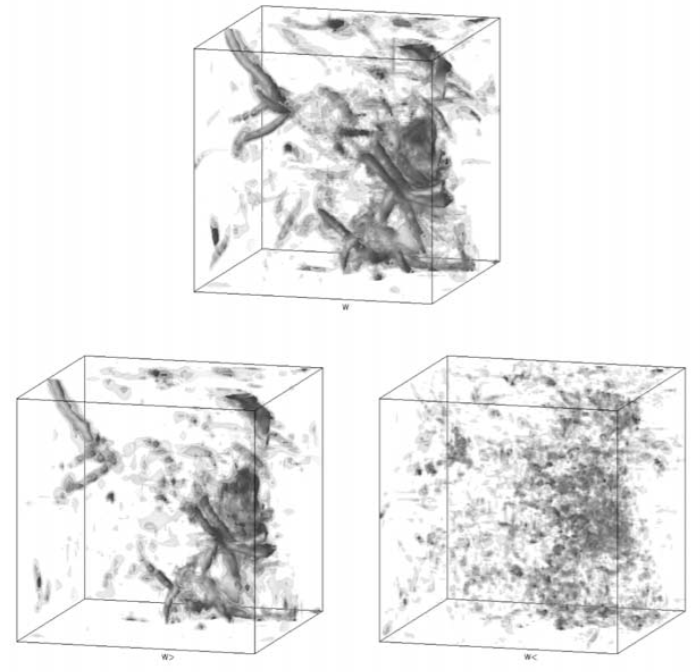
\includegraphics[width=0.65\textwidth]{cvs3}
	\caption{Total (top), coherent (bottom left), and incoherent vorticity (bottom right). Adapted from Farge and Schneider (2001).}
\end{figure}
\end{frame}

%------------------------------------------------

\begin{frame}{Coherent Vortex Simulations (CVS)}

\begin{itemize}
	\item In the original CVS formulation, the separation between coherent and random motions is assumed absolute, with the random part mimicking viscous dissipation
	\item Goldstein and Vasilyev (2004) introduced ``stochastic coherent  adaptive LES'' as a variation on CVS
	\item GV04 use CVS wavelet decomposition, but do not assume that the wavelet filter completely eliminates all the coherent motions from the SFSs
	\item Thus, GV04 assumes that the SFS components themselves contain coherent and random components
\end{itemize}

\end{frame}

%------------------------------------------------

\begin{frame}{A brief overview of wavelet decomposition}

\begin{itemize}
	\item The CVS method uses wavelet decomposition
	\item We will cover a brief overview of wavelets.  For a more detailed view see: 
	\begin{itemize}
		\item Daubechies (1992) -- most recent printing is 2006
		\item Mallat (2009) -- 3rd edition
		\item Farge (1992) -- specific to turbulence research
	\end{itemize}
\end{itemize}

\end{frame}


%------------------------------------------------

\begin{frame}{A brief overview of wavelet decomposition}

\begin{itemize}
	\item With the normal Fourier transform (FT), we assume a periodic function
	\item The FT only tells us what wavenumber (frequency) components exist in a signal
	\item Space (time) and wavenumber (frequency) information cannot be seen at the same time
	\item We need space-wavenumber (time-frequency) representation of a signal
\end{itemize}
\end{frame}

%------------------------------------------------

\begin{frame}{A brief overview of wavelet decomposition}

\begin{itemize}
	\item Why? Real-world signals are non-stationary, meaning it is useful to know if and where some feature happens
	\item A stationary signal has wavenumber (frequency) content unchanged in space (time), and all wavenumber (frequency) components exist everywhere (at all times)
	\item A non-stationary signal changes wavenumbers (frequency) in space (time)
\end{itemize}
\end{frame}

%------------------------------------------------

\begin{frame}{A brief overview of wavelet decomposition}

\begin{itemize}
	\item One early solution is the Short Time (or space) Fourier Transform
\item This technique only analyzes a small portion of signal at a time by using a space or time window -- thus it is often called a Windowed Fourier Transform (WFT)
\item The windowed segment is assumed stationary, and is applied uniformly
\end{itemize}

\end{frame}

%------------------------------------------------

\begin{frame}{A brief overview of wavelet decomposition}
\begin{itemize}
\item Recall, the FT is given by
$$f_k = \frac{1}{2\pi} \int f(x) e^{ikx} dx$$
\item The WFT is applied as
$$f_{k,s} = \frac{1}{2\pi} \int f(s) g(s-x) e^{iks} ds$$
\end{itemize}
where $s$ is the position over a localized region
\end{frame}

%------------------------------------------------

\begin{frame}{A brief overview of wavelet decomposition}
\begin{figure}
	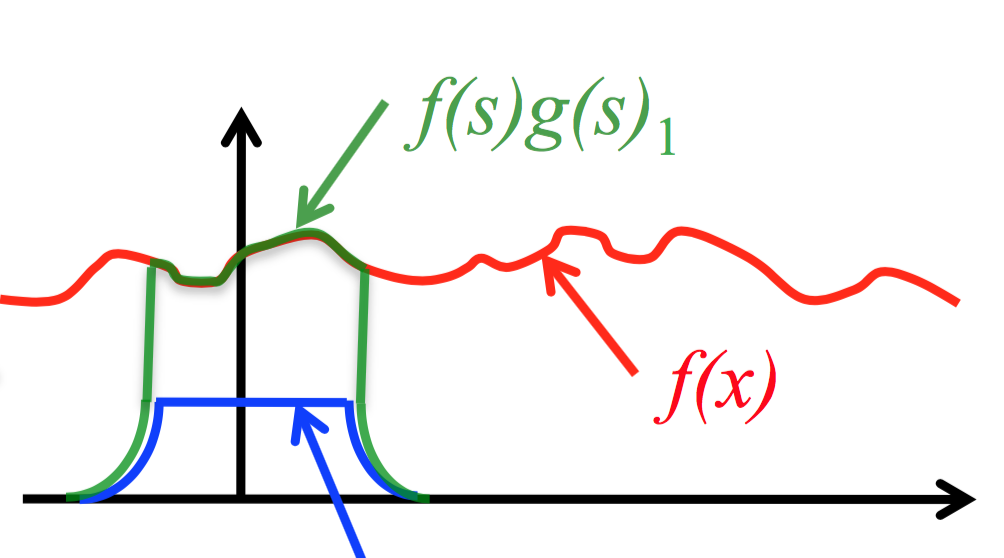
\includegraphics[width=0.65\textwidth]{wavelet1}
\end{figure}
\begin{itemize}
	\item The WFT is our convolution with a filter function in Fourier space
\end{itemize}
\end{frame}

%------------------------------------------------

\begin{frame}{A brief overview of wavelet decomposition}

\begin{itemize}
	\item There are drawbacks to this approach
	\begin{itemize}
		\item The window is unchanged
		\item The resolution dilemma -- a narrow window has poor wavenumber (frequency) resolution, and a wide window has poor spatial (time) resolution
		\item Heisenberg Uncertainty Principle -- we cannot know what wavenumber (frequency) exists at what spatial (time) intervals
	\end{itemize}
\end{itemize}

\end{frame}

%------------------------------------------------

\begin{frame}{A brief overview of wavelet decomposition}

\begin{itemize}
	\item Another approach is called wavelet decomposition
	\item A wavelet is just some small wave
	\item The general idea is to decompose a signal into series of wavelets
	\item This approach helps overcome the resolution dilemma of WFTs
\end{itemize}
\end{frame}

%------------------------------------------------

\begin{frame}{A brief overview of wavelet decomposition}

\begin{itemize}
	\item Wavelets offer an optimal space/frequency decomposition.
	$$W_f(a,b) = |a|^{-\frac{1}{2}} \int f(x) \Psi \left(\frac{x-b}{a}\right)dx$$
	where $\Psi$ is the basis function (``Mother Wavelet''), $b$ translates the basis function, and $a$ scales (dilates) the basis function
	\item A mother wavelet is a prototype for generating the other window functions
\end{itemize}
\end{frame}

%------------------------------------------------

\begin{frame}{A brief overview of wavelet decomposition}

\begin{figure}
	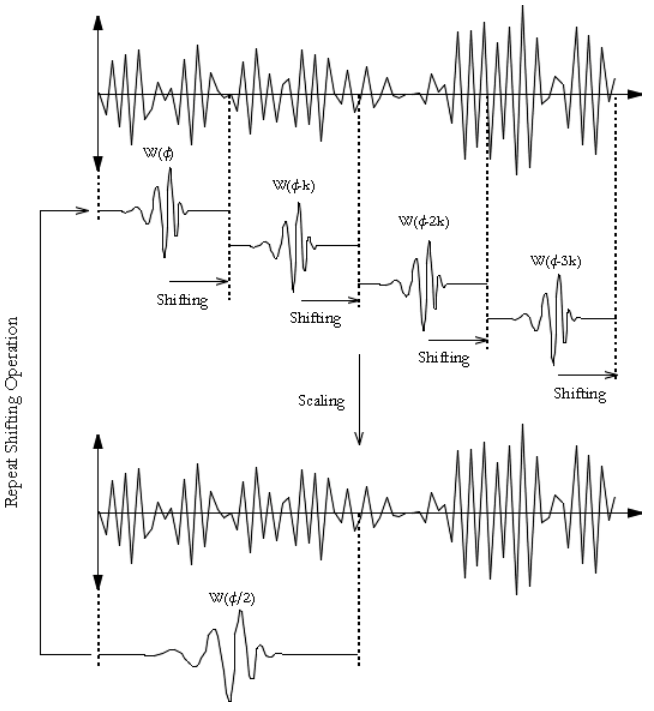
\includegraphics[width=0.6\textwidth]{wavelet5}
	\caption{from wavelet.org}
\end{figure}
\end{frame}

%------------------------------------------------

\begin{frame}{A brief overview of wavelet decomposition}

Common properties of wavelets
\begin{itemize}
	\item A wavelet transform is a set of building blocks to construct or represent a signal  (function)
	\item A wavelet is a 2D expansion set (usually a basis) for a 1D signal
	\item A wavelet expansion gives a space-wavenumber (time-frequency) localization of a signal
	\item The calculation of coefficients can be done efficiently
\end{itemize}
\end{frame}

%------------------------------------------------

\begin{frame}{A brief overview of wavelet decomposition}

Common properties of wavelets
\begin{itemize}
	\item Wavelet systems are generated from a single scaling function (\textit{i.e.} wavelet) by simple scaling and translation
	\item Most useful wavelet systems satisfy the multiresolution condition --  if the basic expansion signals (the wavelets) are made half as wide and translated in steps half  as wide, they will represent a larger class of signals exactly or give a better approximation of any signal
	\item The lower resolution coefficients can be calculated from the higher resolution  coefficients by a tree-structured algorithm
\end{itemize}
\end{frame}

%------------------------------------------------

\begin{frame}{A brief overview of wavelet decomposition}

Multiresolution properties of wavelets
\begin{itemize}
	\item Analyze the signal at different frequencies with different resolutions
	\item Good time resolution and poor frequency resolution at high frequencies
	\item Good frequency resolution and poor time resolution at low frequencies
	\item More suitable for short duration of higher frequency; and longer duration of lower frequency components
\end{itemize}
\end{frame}

%------------------------------------------------

\begin{frame}{A brief overview of wavelet decomposition}

\begin{figure}
	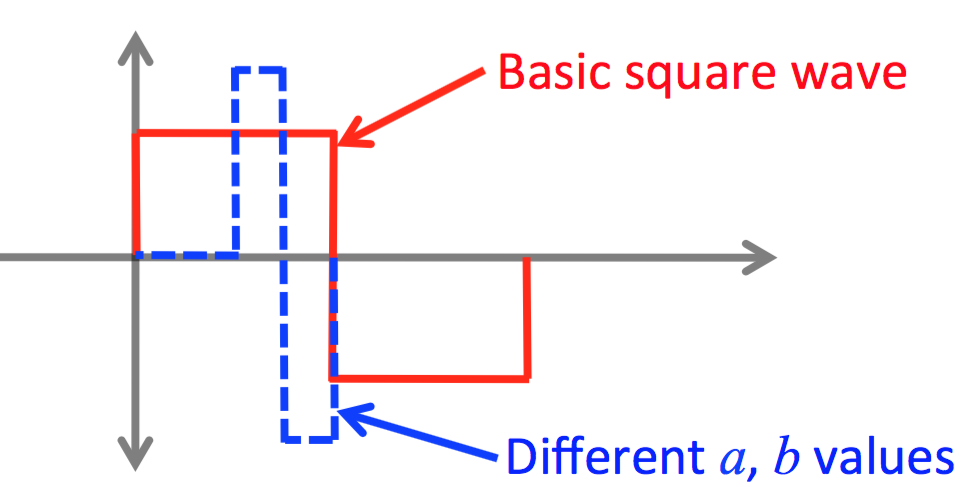
\includegraphics[width=0.6\textwidth]{wavelet2}
\end{figure}

\begin{itemize}
	\item One example of a wavelet is the Haar wavelet (Haar, 1910)
	$$\Psi = \begin{cases} 1 &\mbox{if } 0 \leq x < 0.5 \\ -1 & \mbox{if  } 0.5 \leq x < 1
	\end{cases}$$
\end{itemize}

\end{frame}

%------------------------------------------------

\begin{frame}{A brief overview of wavelet decomposition}


\begin{itemize}
	\item How does wavelet decomposition break down a signal in space and time?
\end{itemize}
\begin{figure}
	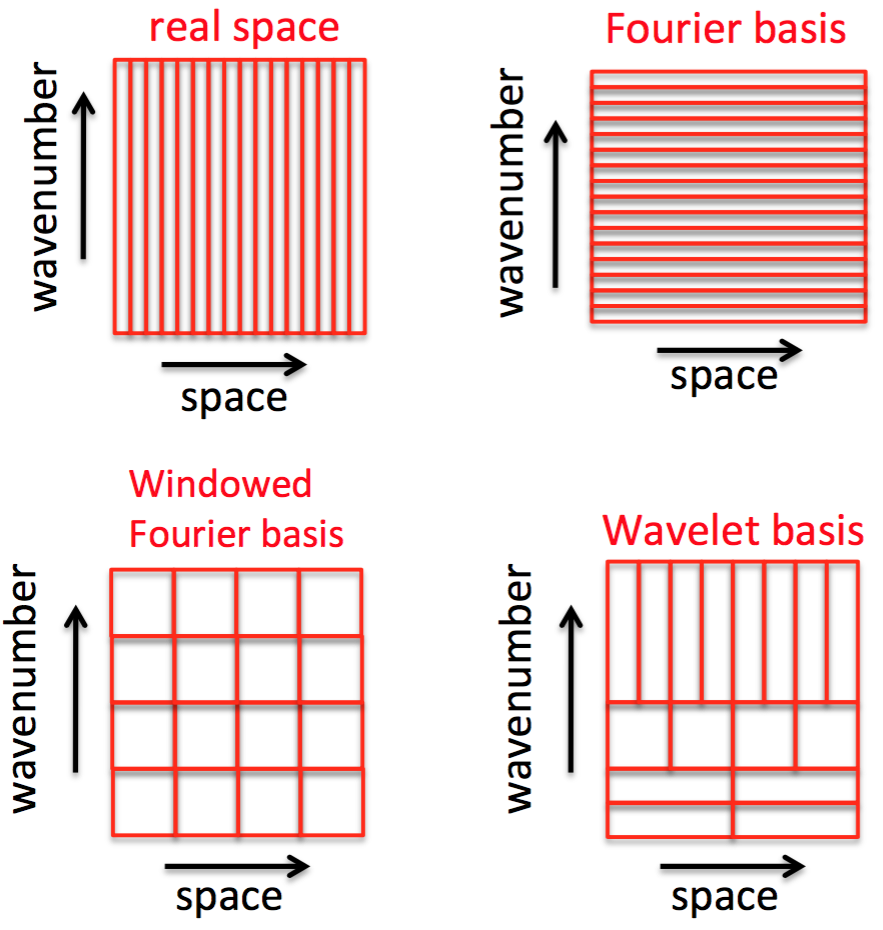
\includegraphics[width=0.6\textwidth]{wavelet3}
\end{figure}

\end{frame}

%------------------------------------------------

\begin{frame}{A brief overview of wavelet decomposition}


\begin{itemize}
	\item The signal is reconstructed by combining $s_i$ and $d_i$ at the desired level ($s$, $ss$, $sss$, etc).
	\begin{itemize}
		\item 1st level – $s_i$ and $d_i$
		\item 2nd level – $ss_i$, $dd_i$, $d_i$
		\item \dots 
	\end{itemize} 
\end{itemize}
\begin{figure}
	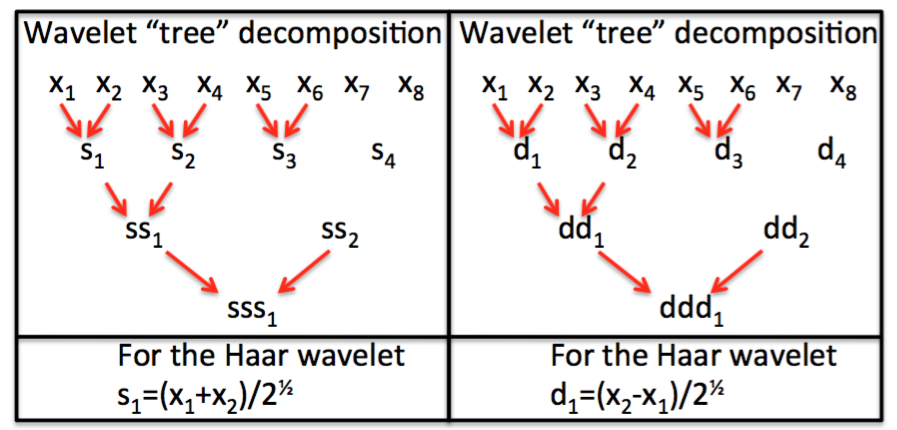
\includegraphics[width=0.75\textwidth]{wavelet4}
\end{figure}

\end{frame}

%------------------------------------------------
\subsection{Filtered Density Functions (FDF)}
%------------------------------------------------

\begin{frame}{Filtered Density Functions (FDF)}

\begin{itemize}
	\item See Colucci et al. (1998) on Canvas or class website
	\item In this method, the evolution of the filtered probability density functions is solved for (\textit{i.e.}, we solve for the evolution of the SFS general moments)
	\item Similar to general PDF transport methods 1st introduced by Lundgren (1969) and outlined in detail in Pope chapter 12.
\end{itemize}

\end{frame}

%------------------------------------------------

\begin{frame}{Filtered Density Functions (FDF)}

\begin{itemize}
	\item Many applications use FDF for scalars in turbulent reacting flows, while traditional equations (low-pass filtered N-S) are solved for momentum (see Fox 2012 for a more detailed discussion)
	\item This type of method is open employed for LES with Lagrangian particle models and for chemically reactive flows
	\item In Lagrangian particle models it leads to a form of the Langevin equations for SFS particle evolution
	\item In chemically reactive flows it has the advantage that the reactions occur in closed form
	\item We will return to these type of methods later in the class when we discuss combining LES with particle models
\end{itemize}

\end{frame}





















































%------------------------------------------------

\end{document}

